% Options for packages loaded elsewhere
\PassOptionsToPackage{unicode}{hyperref}
\PassOptionsToPackage{hyphens}{url}
%
\documentclass[
  man,floatsintext]{apa6}
\usepackage{amsmath,amssymb}
\usepackage{iftex}
\ifPDFTeX
  \usepackage[T1]{fontenc}
  \usepackage[utf8]{inputenc}
  \usepackage{textcomp} % provide euro and other symbols
\else % if luatex or xetex
  \usepackage{unicode-math} % this also loads fontspec
  \defaultfontfeatures{Scale=MatchLowercase}
  \defaultfontfeatures[\rmfamily]{Ligatures=TeX,Scale=1}
\fi
\usepackage{lmodern}
\ifPDFTeX\else
  % xetex/luatex font selection
\fi
% Use upquote if available, for straight quotes in verbatim environments
\IfFileExists{upquote.sty}{\usepackage{upquote}}{}
\IfFileExists{microtype.sty}{% use microtype if available
  \usepackage[]{microtype}
  \UseMicrotypeSet[protrusion]{basicmath} % disable protrusion for tt fonts
}{}
\makeatletter
\@ifundefined{KOMAClassName}{% if non-KOMA class
  \IfFileExists{parskip.sty}{%
    \usepackage{parskip}
  }{% else
    \setlength{\parindent}{0pt}
    \setlength{\parskip}{6pt plus 2pt minus 1pt}}
}{% if KOMA class
  \KOMAoptions{parskip=half}}
\makeatother
\usepackage{xcolor}
\usepackage{graphicx}
\makeatletter
\def\maxwidth{\ifdim\Gin@nat@width>\linewidth\linewidth\else\Gin@nat@width\fi}
\def\maxheight{\ifdim\Gin@nat@height>\textheight\textheight\else\Gin@nat@height\fi}
\makeatother
% Scale images if necessary, so that they will not overflow the page
% margins by default, and it is still possible to overwrite the defaults
% using explicit options in \includegraphics[width, height, ...]{}
\setkeys{Gin}{width=\maxwidth,height=\maxheight,keepaspectratio}
% Set default figure placement to htbp
\makeatletter
\def\fps@figure{htbp}
\makeatother
\setlength{\emergencystretch}{3em} % prevent overfull lines
\providecommand{\tightlist}{%
  \setlength{\itemsep}{0pt}\setlength{\parskip}{0pt}}
\setcounter{secnumdepth}{-\maxdimen} % remove section numbering
% Make \paragraph and \subparagraph free-standing
\ifx\paragraph\undefined\else
  \let\oldparagraph\paragraph
  \renewcommand{\paragraph}[1]{\oldparagraph{#1}\mbox{}}
\fi
\ifx\subparagraph\undefined\else
  \let\oldsubparagraph\subparagraph
  \renewcommand{\subparagraph}[1]{\oldsubparagraph{#1}\mbox{}}
\fi
\newlength{\cslhangindent}
\setlength{\cslhangindent}{1.5em}
\newlength{\csllabelwidth}
\setlength{\csllabelwidth}{3em}
\newlength{\cslentryspacingunit} % times entry-spacing
\setlength{\cslentryspacingunit}{\parskip}
\newenvironment{CSLReferences}[2] % #1 hanging-ident, #2 entry spacing
 {% don't indent paragraphs
  \setlength{\parindent}{0pt}
  % turn on hanging indent if param 1 is 1
  \ifodd #1
  \let\oldpar\par
  \def\par{\hangindent=\cslhangindent\oldpar}
  \fi
  % set entry spacing
  \setlength{\parskip}{#2\cslentryspacingunit}
 }%
 {}
\usepackage{calc}
\newcommand{\CSLBlock}[1]{#1\hfill\break}
\newcommand{\CSLLeftMargin}[1]{\parbox[t]{\csllabelwidth}{#1}}
\newcommand{\CSLRightInline}[1]{\parbox[t]{\linewidth - \csllabelwidth}{#1}\break}
\newcommand{\CSLIndent}[1]{\hspace{\cslhangindent}#1}
\ifLuaTeX
\usepackage[bidi=basic]{babel}
\else
\usepackage[bidi=default]{babel}
\fi
\babelprovide[main,import]{english}
% get rid of language-specific shorthands (see #6817):
\let\LanguageShortHands\languageshorthands
\def\languageshorthands#1{}
% Manuscript styling
\usepackage{upgreek}
\captionsetup{font=singlespacing,justification=justified}

% Table formatting
\usepackage{longtable}
\usepackage{lscape}
% \usepackage[counterclockwise]{rotating}   % Landscape page setup for large tables
\usepackage{multirow}		% Table styling
\usepackage{tabularx}		% Control Column width
\usepackage[flushleft]{threeparttable}	% Allows for three part tables with a specified notes section
\usepackage{threeparttablex}            % Lets threeparttable work with longtable

% Create new environments so endfloat can handle them
% \newenvironment{ltable}
%   {\begin{landscape}\centering\begin{threeparttable}}
%   {\end{threeparttable}\end{landscape}}
\newenvironment{lltable}{\begin{landscape}\centering\begin{ThreePartTable}}{\end{ThreePartTable}\end{landscape}}

% Enables adjusting longtable caption width to table width
% Solution found at http://golatex.de/longtable-mit-caption-so-breit-wie-die-tabelle-t15767.html
\makeatletter
\newcommand\LastLTentrywidth{1em}
\newlength\longtablewidth
\setlength{\longtablewidth}{1in}
\newcommand{\getlongtablewidth}{\begingroup \ifcsname LT@\roman{LT@tables}\endcsname \global\longtablewidth=0pt \renewcommand{\LT@entry}[2]{\global\advance\longtablewidth by ##2\relax\gdef\LastLTentrywidth{##2}}\@nameuse{LT@\roman{LT@tables}} \fi \endgroup}

% \setlength{\parindent}{0.5in}
% \setlength{\parskip}{0pt plus 0pt minus 0pt}

% Overwrite redefinition of paragraph and subparagraph by the default LaTeX template
% See https://github.com/crsh/papaja/issues/292
\makeatletter
\renewcommand{\paragraph}{\@startsection{paragraph}{4}{\parindent}%
  {0\baselineskip \@plus 0.2ex \@minus 0.2ex}%
  {-1em}%
  {\normalfont\normalsize\bfseries\itshape\typesectitle}}

\renewcommand{\subparagraph}[1]{\@startsection{subparagraph}{5}{1em}%
  {0\baselineskip \@plus 0.2ex \@minus 0.2ex}%
  {-\z@\relax}%
  {\normalfont\normalsize\itshape\hspace{\parindent}{#1}\textit{\addperi}}{\relax}}
\makeatother

\makeatletter
\usepackage{etoolbox}
\patchcmd{\maketitle}
  {\section{\normalfont\normalsize\abstractname}}
  {\section*{\normalfont\normalsize\abstractname}}
  {}{\typeout{Failed to patch abstract.}}
\patchcmd{\maketitle}
  {\section{\protect\normalfont{\@title}}}
  {\section*{\protect\normalfont{\@title}}}
  {}{\typeout{Failed to patch title.}}
\makeatother

\usepackage{xpatch}
\makeatletter
\xapptocmd\appendix
  {\xapptocmd\section
    {\addcontentsline{toc}{section}{\appendixname\ifoneappendix\else~\theappendix\fi\\: #1}}
    {}{\InnerPatchFailed}%
  }
{}{\PatchFailed}
\keywords{Canine; Dog; Interspecies interaction; Pointing; Social communication}
\usepackage{lineno}

\linenumbers
\usepackage{csquotes}
\usepackage{pdflscape}
\ifLuaTeX
  \usepackage{selnolig}  % disable illegal ligatures
\fi
\IfFileExists{bookmark.sty}{\usepackage{bookmark}}{\usepackage{hyperref}}
\IfFileExists{xurl.sty}{\usepackage{xurl}}{} % add URL line breaks if available
\urlstyle{same}
\hypersetup{
  pdftitle={Data from ManyDogs 1},
  pdfauthor={ManyDogs Project, Julia Espinosa1, Elizabeth Hare2, Daniela Alberghina3, Bryan Mitchel Perez Valverde4, \& Jeffrey R. Stevens5},
  pdflang={en-EN},
  pdfkeywords={Canine; Dog; Interspecies interaction; Pointing; Social communication},
  hidelinks,
  pdfcreator={LaTeX via pandoc}}

\title{Data from ManyDogs 1}
\author{ManyDogs Project\textsuperscript{}, Julia Espinosa\textsuperscript{1}, Elizabeth Hare\textsuperscript{2}, Daniela Alberghina\textsuperscript{3}, Bryan Mitchel Perez Valverde\textsuperscript{4}, \& Jeffrey R. Stevens\textsuperscript{5}}
\date{}


\shorttitle{Data from ManyDogs 1}

\authornote{

Correspondence concerning this article should be addressed to Jeffrey R. Stevens, B83 East Stadium, University of Nebraska-Lincoln, Lincoln, Nebraska 68588, USA. E-mail: \href{mailto:jeffrey.r.stevens@gmail.com}{\nolinkurl{jeffrey.r.stevens@gmail.com}}

}

\affiliation{\vspace{0.5cm}\textsuperscript{1} Department of Human Evolutionary Biology, Harvard University, Cambridge, MA, USA\\\textsuperscript{2} Dog Genetics LLC, Astoria, NY, USA\\\textsuperscript{3} Department of Veterinary Sciences, University of Messina, Messina, Italy\\\textsuperscript{4} The Graduate Center, City University of New York, New York City, New York, USA\\\textsuperscript{5} Department of Psychology, Center for Brain, Biology \& Behavior, University of Nebraska-Lincoln, Lincoln, Nebraska, USA}

\abstract{%
The ManyDogs 1 study is the first multi-site collaborative study of dogs' responses to human pointing. It addressed whether dogs perceive the gesture as socially communicative and are therefore more likely to follow the point when it is paired with additional social signals (ManyDogs Project, et al., 2023b). Researchers from 20 research sites across eight countries collected data from 704 dogs. Here, we present not only the behavior data on the dogs' responses to experimental pointing conditions but also guardian responses to survey questions, including the Canine Behavior and Research Questionnaire (C-BARQ©, Hsu and Serpell, 2003). This dataset allows for assessing associations among C-BARQ measures as well as connections to the experimental task data, research site metadata, and other dog and guardian characteristic data.
}



\begin{document}
\maketitle

\hypertarget{background}{%
\subsection{(1) Background}\label{background}}

ManyDogs is an international research consortium of scientists with a shared interest in the factors driving canine behavior and cognition (ManyDogs Project et al., 2023a). This consortium actively fosters a diverse community and formalizes a transparent and equitable process for engaging in multi-site collaborative projects related to canine behavior and cognition. In the first ManyDogs study---named ManyDogs 1 (ManyDogs Project et al., 2023b), we investigated a question of theoretical importance in canine science: Do dogs act on human pointing signals as though they are communicative social cues? Domestic dogs (\emph{Canis familiaris}) have become a popular animal model for investigating behavioral and cognitive evolution due to their shared ecological niche with humans and because they are plentiful, easy-to-access research subjects in many parts of the world. Interest in their putatively innate ability to interact and cooperate with humans has made them particularly popular in comparative studies, especially as they appear to respond to human communicative cues---such as pointing---more accurately and flexibly than other species (e.g., Bräuer et al., 2006). Though point following behavior in dogs has been widely observed and studied over recent decades (Miklösi et al., 1998; Soproni et al., 2001; Hare et al., 2002; Kaminski \& Nitzschner, 2013), there is still disagreement as to the underlying motivation for the behavior. Do dogs respond to pointing because they interpret the gesture as socially communicative (Hare \& Tomasello, 1999; Soproni et al., 2001; Kaminski \& Nitzschner, 2013)? Or rather, because dogs have learned to associate human pointing with food rewards (e.g., Wynne et al., 2008)?

To investigate this question, we used a big team science, single-study approach, modeled after other groups such as ManyBabies (Frank et al., 2017) and ManyPrimates (ManyPrimates et al., 2019). With this method, multiple research teams followed the same experimental protocol, sharing the high cost of behavioral data collection and striving to implement the method in an identical manner. This approach replicated the study simultaneously in different research environments and with different populations.

Under our main hypothesis, we predicted that when dogs saw a pointing gesture paired with \emph{ostensive} signals, such as eye gaze and dog-directed speech (i.e., calling the dog's name), they would be more likely to follow the gesture than when no such ostensive cues accompanied the point. If we observed this response across dogs, the result would lend support to the idea that explicitly communicative cues help dogs understand the intention behind the gesture. Such an outcome would suggest that dogs find ostensive cues necessary for understanding pointing, similar to human children (Behne et al., 2005). On the other hand, if no difference was observed in point following across the ostensive and non-ostensive conditions (pointing without additional cues), this outcome would suggest that dogs indiscriminately follow pointing. Such a result would suggest that dogs raised by humans may learn to associate pointing limbs with rewards and not necessarily perceive any communicative intention underlying the gesture.

In addition to testing our main hypothesis, we took the opportunity offered by multiple research teams in different sites collaborating on the same study to collect data on sources of inter-site variability that could influence the results. Often, studies by different groups produce inconsistent results (Rodriguez et al., 2021). The impact of cultural differences in scientific practice, dog training norms across regions, and of course variation in heritable traits across dog breeds have complicated replication studies conducted by isolated groups, making it difficult to pinpoint the reasons that results differ. By collecting extensive and detailed information about the testing environments and subject population, we achieved a rich and robust dataset that would support investigation about multiple influences on dogs' behavior previously out of reach.

\hypertarget{methods}{%
\subsection{(2) Methods}\label{methods}}

\hypertarget{study-design}{%
\subsection{2.1 Study design}\label{study-design}}

The ManyDogs 1 study used a cross-sectional, multi-method approach to collecting data. Dog guardians were recruited through the individual research sites' existing databases and via their respective outreach methods (e.g., social media). Prior to participating in the behavioral tasks at a research site, guardians completed an online survey, providing basic environment and demographic information along with a validated assessment of canine temperament and behavior---the Canine Behavioral Assessment and Research Questionnaire (C-BARQ©, Hsu \& Serpell, 2003). The behavioral tasks included a short series of object-choice warm-ups that acclimated the dog to the space, followed by two experimental pointing conditions. Using a within-subjects design, dogs were tested on two different pointing cues by a trained researcher, ostensive and non-ostensive, in counterbalanced orders across subjects. Response rates to these two styles of pointing were compared within subjects, while additional between-subject variables derived from the survey data supported investigating variability in behavior as a function of demographic and environmental factors.

\hypertarget{time-of-data-collection}{%
\subsection{2.2 Time of data collection}\label{time-of-data-collection}}

Data for the study were collected over 13 months, between January 2022 and January 2023. Within this time window, research sites were able to decide when to implement the protocol according to the guardian and staff availability (collection dates available in dataset).

\hypertarget{location-of-data-collection}{%
\subsection{2.3 Location of data collection}\label{location-of-data-collection}}

For the main study, data were collected in 20 research sites across eight countries (Argentina, Canada, Croatia, Hungary, Italy, Poland, UK, USA) on three continents (Figure \ref{fig:countries}). In addition, an Austrian site recorded only pilot data and is not represented in this dataset. A full list and description of research sites is available in Table S1 of ManyDogs Project et al. (2023b).

\begin{figure}

{\centering 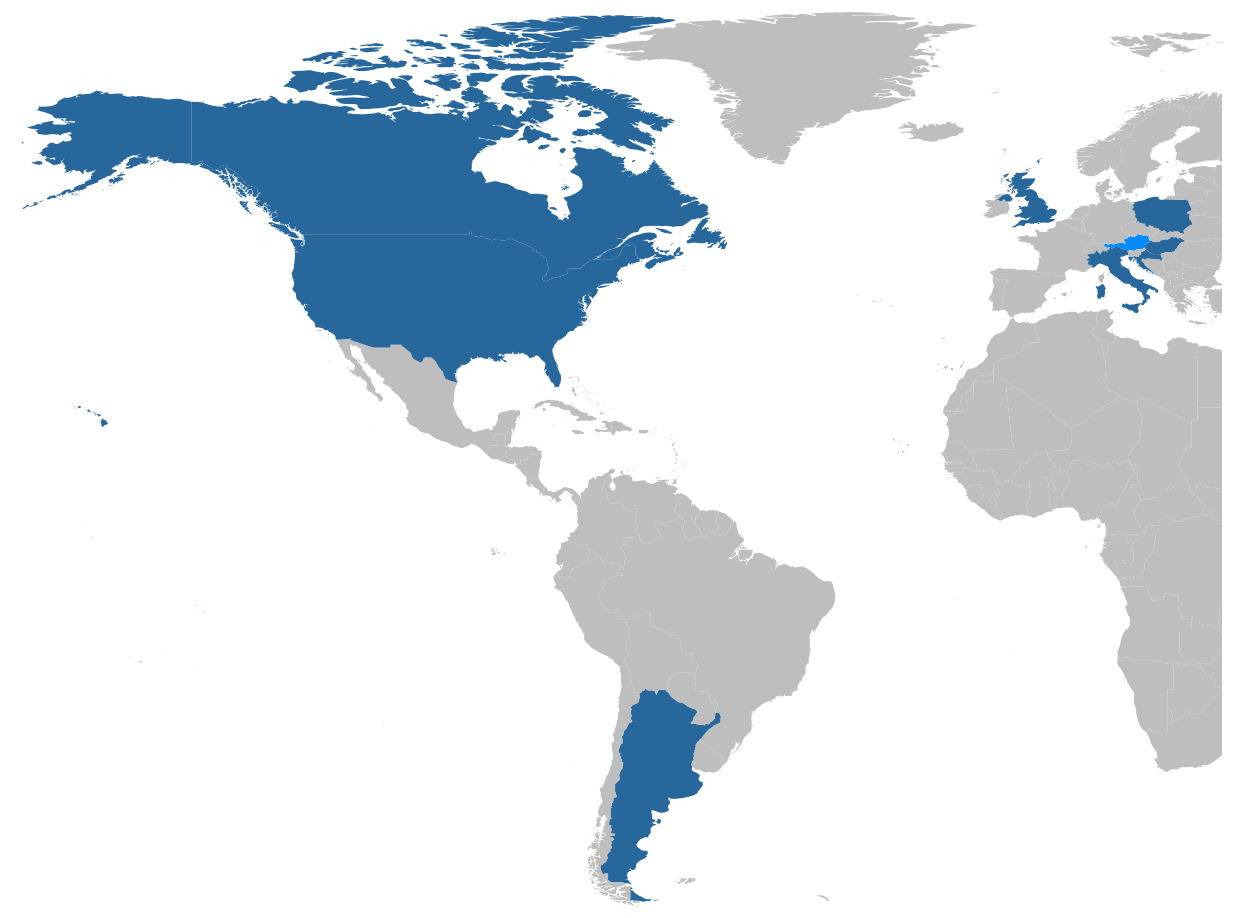
\includegraphics[width=0.8\linewidth]{md1_countries} 

}

\caption{ManyDogs 1 data presented here were collected from 20 research sites in eight countries: Argentina, Canada, Croatia, Hungary, Italy, Poland, UK, USA. Pilot data not included in this dataset were collected from a site in Austria.}\label{fig:countries}
\end{figure}

\hypertarget{sampling-sample-and-data-collection}{%
\subsection{2.4 Sampling, sample and data collection}\label{sampling-sample-and-data-collection}}

Across all sites, teams behaviorally tested 704 dogs (M:F = 334:373, mean ± SD age = 4.40 ± 3.1 years {[}range = 0.3-20.8{]}). Approximately 76.9\% of the dogs were spayed or neutered, 53.8\% were of single-breed ancestry (comprising 85 distinct breeds), 90.2\% lived in private homes, 9.6\% lived in group/kennel housing, and 0.3\% lived in other housing. Complete behavioral data were collected from 455 dogs, and complete survey data were collected from 495 dogs. Guardians identified as female (81.0\%), male (17.7\%), and nonbinary/other (1.3\%) with a modal guardian age range of 30-39 years.

\hypertarget{materialssurvey-instruments}{%
\subsection{2.5 Materials/Survey instruments}\label{materialssurvey-instruments}}

The guardian survey was hosted on Qualtrics (complete survey available at \url{https://doi.org/10.17605/OSF.IO/7RWPC/}). The survey included dog demographics (name, living situation, sex, neuter status, birth date, breed information, acquisition type), training information (communication style and frequency, training experience, research experience), guardian demographics (gender, age, community type), and C-BARQ. The C-BARQ trainability scale (eight items) was presented first and was included in the pre-registered analysis of pointing (ManyDogs Project et al., 2023b). After answering the trainability questions, guardians could decide to submit their responses or continue to complete the remaining six behavior assessment scales. If they continued, they answered questions about aggression (28 questions), fear (18 questions), separation-related behavior (9 questions), excitability (7 questions), attachment/attention-seeking (7 questions), and miscellaneous behavior problems (28 questions), including chasing, chewing, begging, pulling, urinating, defecating, barking, and licking. Most questions used a 5-point Likert scale with a Not Observed option. Some categories included open-ended questions for additional explanations of their dog's behavior, but we did not include them in our dataset to protect guardian anonymity.

Behavioral data were collected at individual research sites, where guardians brought the dogs in for test sessions. After the dogs acclimated to the testing room, they completed a series of warm-up object-choice tasks in which food was hidden under cups and they had to approach a cup to receive any food rewards hidden underneath (complete methods available in ManyDogs Project et al., 2023b). These tests were conducted by two individuals: an experimenter to bait and place the cups and a handler to release the dog to make a choice and recall for subsequent trials (handlers could be either trained researchers or the dog's guardian).

Sessions started with warm-up trials to familiarize the dogs to the testing procedures. These involved trying to find a food reward placed under a single cup (one-cup warm-ups with four out of seven trials correct) or under one of two cups (two-cup warm-ups with four out of size trials correct). Once meeting the completion criteria, the dogs moved on to two experimental condition sessions with eight trials per condition (condition order counterbalanced between subjects). In the non-ostensive condition, the experimenter cleared their throat to get the dog's attention, showed them the food, and placed food underneath one of two cups behind a visual barrier. They then removed the barrier, gazed at the ground in front of them, cleared their throat again, and pointed to the cup with the food using a contralateral momentary point. In the ostensive condition, instead of clearing their throat, the experimenter said ``{[}dog name{]}, look!'' in an engaging voice and they made eye contact with the subject instead of looking at the floor. The two conditions were separated by a one-minute play break and re-familiarization with the testing situation. After the two experimental conditions, the dogs completed an odor control condition with a similar set-up as the ostensive condition, except no point cue was given. The control was intended to determine whether the dogs were using olfactory instead of visual cues to solve the task.

\hypertarget{quality-control}{%
\subsection{2.6 Quality control}\label{quality-control}}

Collecting high-quality data was a key objective of ManyDogs 1. To validate the study design and analysis plan, we conducted a pilot experiment at a single site with 91 dogs. We pre-registered the pilot study at the Open Science Framework (\url{https://osf.io/gz5pj/}). The pilot data are not included in this dataset.

For the primary study presented here, we pre-registered the hypotheses, methods, and analysis plan as a registered report at \emph{Animal Behavior and Cognition} (\url{https://doi.org/10.31234/osf.io/f86jq}). Because this study involved multiple sites running the same protocol, we sought to ensure consistent implementation across sites. During a researcher training phase, participating sites were required to submit videos of their team performing the protocol, as well as the full set of videos from the first dog tested. Two project administrators reviewed the videos for all sites and provided feedback on each site's implementation to improve consistency across sites.

Behavioral tests were video recorded and experimenters also live-coded the dog's responses on paper. Data were compiled across sites through a data entry survey hosted on Qualtrics. Using a survey protected the resulting data file from errors associated with directly editing the file. To measure inter-rater reliability of the live coding of experimental sessions, each site had a research assistant blind to the project's focus recode a subset of sessions. This recoding resulted in an overall Cohen's kappa of 0.98 with individual sites ranging from kappa = 0.92-1.00.

\hypertarget{data-anonymization-and-ethical-issues}{%
\subsection{2.7 Data anonymization and ethical issues}\label{data-anonymization-and-ethical-issues}}

Each research site participating in this study obtained approval from their respective institutional ethics committee (see Table S1 of ManyDogs Project et al., 2023b). All guardians gave informed consent to participate and were free to discontinue from the study at any time.

All identifiable information has been removed from the dataset, including replacing dog names with ID numbers.

\hypertarget{existing-use-of-data}{%
\subsection{2.8 Existing use of data}\label{existing-use-of-data}}

A portion of the guardian data collected for the ManyDogs 1 study was used and published in:

ManyDogs Project, Espinosa, J., Stevens, J.R., Alberghina, D., Barela, J., Bogese, M., Bray, E., Buchsbaum, D., Byosiere, S.-E., Cavalli, C., Dror, S., Fitzpatrick, H., Freeman, M.S., Frinton, S., Gnanadesikan, G., Guran, C.-N.A., Glover, M., Hare, B., Hare, E., Hickey, M., Horschler, D., Huber, L., Jim, H.-L., Johnston, A., Kaminski, J., Kelly, D., Kuhlmeier, V.A., Lassiter, L., MacLean, E., Ostojic, L., Pelgrim, M.H., Pellowe, S., Salomons, H., Santos, L., Silver, Z.A., Silverman, J.M., Sommese, A., Völter, C., Walsh, C.,
Worth, Y.A., Zipperling, L.M.I., Żołędziewska, B., and Zylberfuden, S. G. (2023). ManyDogs 1: A multi-lab replication study of dogs' pointing comprehension. \emph{Animal Behavior and Cognition}, 10(3), 232-286.
\url{https://doi.org/10.26451/abc.10.03.03.2023}

\hypertarget{dataset-description-and-access}{%
\subsection{(3) Dataset description and access}\label{dataset-description-and-access}}

The dataset contains 704 observations of 158 variables described in a codebook and Table \ref{tab:displayDescription}. The dataset contains variables supplied by a survey as well as experimental variables. Data provided by each dog's guardian include demographic information about the dog and guardian, responses to questions about the types and frequencies of the dog's training activities, and answers to the C-BARQ.

In addition to the data provided by guardians, experimental variables are included in this dataset. These include information about experimental conditions, proportions of correct choices under ostensive and non-ostensive conditions, whether the correct and chosen option were on the right side of the dog, and whether the dog completed the experiment and was used in the analysis.

\hypertarget{repository-location}{%
\subsection{3.1 Repository location}\label{repository-location}}

The dataset for this study is available on the Open Science Framework at \url{https://osf.io/7rwpc/} (DOI: \href{https://doi.org/10.17605/OSF.IO/7RWPC}{10.17605/OSF.IO/7RWPC}) and on GitHub at \url{https://github.com/ManyDogsProject/md1_datapaper}.

\hypertarget{objectfile-name}{%
\subsection{3.2 Object/file name}\label{objectfile-name}}

The file name for the dataset is \texttt{manydogs\_etal\_2024\_data.csv} and the codebook is \texttt{manydogs\_etal\_2024\_codebook.csv}.

\hypertarget{data-type}{%
\subsection{3.3 Data type}\label{data-type}}

This dataset includes processed data from the ManyDogs 1 study. We have removed identifiable information, recoded data values for consistency, renamed and reordered columns for clarity, and combined survey data submitted by guardians via Qualtrics and behavioral data submitted by research teams via Qualtrics.

\hypertarget{format-names-and-versions}{%
\subsection{3.4 Format names and versions}\label{format-names-and-versions}}

The dataset and codebook are provided in a comma-separated (\texttt{.csv}) plain text format. There is one version of the dataset with no anticipated additional versions, as data collection has ended.

\hypertarget{language}{%
\subsection{3.5 Language}\label{language}}

The variable names and text values are in English. Though data were collected in other languages (Croatian, Hungarian, Italian, Polish, and Spanish), the Qualtrics surveys were coded to save responses in English.

\hypertarget{license}{%
\subsection{3.6 License}\label{license}}

The ManyDogs 1 dataset is available under a \href{https://creativecommons.org/licenses/by/4.0/}{CC BY 4.0 license}, which allows users to share (copy and redistribute the material in any medium or format for any purpose, even commercially) and adapt (remix, transform, and build upon the material for any purpose, even commercially) this material as long as they give appropriate credit, provide a link to the license, indicate if changes were made, and do not apply legal terms or technological measures that legally restrict others from doing anything the license permits.

\hypertarget{limits-to-sharing}{%
\subsection{3.7 Limits to sharing}\label{limits-to-sharing}}

The dataset is freely available for download on the \href{https://doi.org/10.17605/OSF.IO/7RWPC}{Open Science Framework}. There are no limits to sharing beyond those described in the license.

\hypertarget{publication-date}{%
\subsection{3.8 Publication date}\label{publication-date}}

The dataset was uploaded to the \href{https://doi.org/10.17605/OSF.IO/7RWPC}{Open Science Framework} on 2024-02-06.

\hypertarget{fair-datacodebook}{%
\subsection{3.9 FAIR data/Codebook}\label{fair-datacodebook}}

This dataset is \emph{findable} through the persistent identifier on the Open Science Framework (DOI: \href{https://doi.org/10.17605/OSF.IO/7RWPC}{10.17605/OSF.IO/7RWPC}), \emph{accessible} through free availability on Open Science Framework and GitHub, \emph{interoperable} by using plain-text CSV data files, and \emph{reusable} with the CC-BY 4.0 license. Metadata are included as codebook here (Table \ref{tab:displayDescription}) and with the data on Open Science Framework and GitHub.

\hypertarget{reuse-potential}{%
\subsection{(4) Reuse potential}\label{reuse-potential}}

The original data from ManyDogs 1 (ManyDogs Project et al., 2023b) focuses on dog responses in the two-alternative object-choice task across warm-up, ostenstive, non-ostenstive, and odor control trials. In addition, that dataset includes basic demographics on the dog and guardian, as well as the mean trainability score from the C-BARQ. The current dataset adds information on dog origin and household, dog training experience, guardian communication practices, and the complete C-BARQ profile. The C-BARQ data are quite rich, with sections on training, aggression, fear, separation-related behavior, excitability, attachment and attention seeking, and miscellaneous problem behaviors. Thus, this dataset allows for assessing associations among all of the C-BARQ measures as well as connections to the experimental task data and the other dog and guardian characteristic data.

A key strength of this dataset is its diversity. The data were collected by 20 different research sites in eight countries, allowing the assessment of site effects as well as cultural differences. In addition, while most dogs are kept in private homes, the dataset also includes a subset of dogs kept in group housing at working dog facilities. Finally, breed is included, allowing the exploration of breed differences.

Though the current dataset has expanded survey information about dog and guardian characteristics, the behavioral task data have been summarized at the level of mean choices per subject and experimental condition rather than including individual trial data. Thus, the trial data are not available for analysis in the current dataset. However, the trial data are available in the original dataset, so it is possible to merge the current and original datasets using dog ID as the primary key to gain access to the trial data. An additional limitation is that, though the C-BARQ training survey questions were compulsory for all guardians, the remaining questions were optional to ease the survey burden. As a result, 512 of the 704 guardians elected to continue on to the optional questions (though not all completed the survey).

\hypertarget{contribution-statement}{%
\subsection{Contribution Statement}\label{contribution-statement}}

The authors made the following contributions. Julia Espinosa: Conceptualization, Data curation, Formal analysis, Funding acquisition, Methodology, Project administration, Supervision, Writing - original draft, Writing - review \& editing; Elizabeth Hare: Conceptualization, Data curation, Formal analysis, Methodology, Project administration, Software, Validation, Writing - original draft, Writing - review \& editing; Daniela Alberghina: Investigation, Validation, Writing - original draft, Writing - review \& editing; Brian Perez: Investigation, Validation, Writing - original draft, Writing - review \& editing; Jeffrey R. Stevens: Conceptualization, Data curation, Formal analysis, Methodology, Project administration, Software, Supervision, Visualization, Writing - original draft, Writing - review \& editing.

For the original ManyDogs 1 study, data were collected by: D. Alberghina., H.E.E. Alway, J.D. Barela, E.E. Bray, S.-E. Byosiere, C.M. Cavalli, L.M. Chaudoir, C. Collins-Pisano, H.J. DeBoer, L.E.L.C. Douglas, S. Dror, M.V. Dzik, B. Ferguson, L. Fisher, H.C. Fitzpatrick, M.S. Freeman, S.N. Frinton, M.K. Glover, J.E.P. Goacher, M. Golańska, M.
Hickey, H.-L. Jim, D.M. Kelly, V.A. Kuhlmeier, L. Lassiter, L. Lazarowski, J. Leighton-Birch, K. Maliszewska, V. Marra, L.I. Montgomery, M.S. Murray, E.K. Nelson, L. Ostojić, S.G. Palermo, A.E. Parks Russell, M.H. Pelgrim, S.D. Pellowe, A. Reinholz, L.A. Rial, E.M. Richards, M.A.~Ross, L.G. Rothkoff, H.Salomons, J.K. Sanger, A.R. Schirle, S.J. Shearer, J.M. Silverman, A. Sommese, T. Srdoc, H. St.~John-Mosse, K. Vékony, Y.A. Worth, L.M.I. Zipperling, B. Żołędziewska, and S.G. Zylberfuden.

\hypertarget{acknowledgments}{%
\subsection{Acknowledgments}\label{acknowledgments}}

We are grateful to all of the research teams and dog guardians who helped generate these data. We are grateful to James Serpell for allowing us to use the C-BARQ questionnaire.

\hypertarget{conflict-of-interest}{%
\subsection{Conflict of Interest}\label{conflict-of-interest}}

The author(s) declare no conflict of interest associated with the publication of this manuscript.

\hypertarget{funding-statement}{%
\subsection{Funding statement}\label{funding-statement}}

We are grateful to the Big Team Science Conference for funding the article processing fee via a grant to JE.

\newpage

\hypertarget{references}{%
\section{References}\label{references}}

\hypertarget{refs}{}
\begin{CSLReferences}{1}{0}
\leavevmode\vadjust pre{\hypertarget{ref-Behne.etal.2005}{}}%
Behne, T., Carpenter, M., \& Tomasello, M. (2005). One-year-olds comprehend the communicative intentions behind gestures in a hiding game. \emph{Developmental Science}, \emph{8}(6), 492--499. \url{https://doi.org/10.1111/j.1467-7687.2005.00440.x}

\leavevmode\vadjust pre{\hypertarget{ref-Brauer.etal.2006}{}}%
Bräuer, J., Kaminski, J., Riedel, J., Call, J., \& Tomasello, M. (2006). Making inferences about the location of hidden food: {Social} dog, causal ape. \emph{Journal of Comparative Psychology}, \emph{120}(1), 38--47. \url{https://doi.org/10.1037/0735-7036.120.1.38}

\leavevmode\vadjust pre{\hypertarget{ref-Frank.etal.2017}{}}%
Frank, M. C., Bergelson, E., Bergmann, C., Cristia, A., Floccia, C., Gervain, J., Hamlin, J. K., Hannon, E. E., Kline, M., Levelt, C., Lew-Williams, C., Nazzi, T., Panneton, R., Rabagliati, H., Soderstrom, M., Sullivan, J., Waxman, S., \& Yurovsky, D. (2017). A collaborative approach to infant research: Promoting reproducibility, best practices, and theory-building. \emph{Infancy}, \emph{22}(4), 421--435. \url{https://doi.org/10.1111/infa.12182}

\leavevmode\vadjust pre{\hypertarget{ref-Hare.etal.2002}{}}%
Hare, B., Brown, M., Williamson, C., \& Tomasello, M. (2002). The domestication of social cognition in dogs. \emph{Science}, \emph{298}, 1634--1636.

\leavevmode\vadjust pre{\hypertarget{ref-Hare.Tomasello.1999}{}}%
Hare, B., \& Tomasello, M. (1999). Domestic dogs (\emph{{Canis} familiaris}) use human and conspecific social cues to locate hidden food. \emph{Journal of Comparative Psychology}, \emph{113}(2), 173--177. \url{https://doi.org/10.1037/0735-7036.113.2.173}

\leavevmode\vadjust pre{\hypertarget{ref-Hsu.Serpell.2003}{}}%
Hsu, Y., \& Serpell, J. A. (2003). Development and validation of a questionnaire for measuring behavior and temperament traits in pet dogs. \emph{Journal of the American Veterinary Medical Association}, \emph{223}(9), 1293--1300. \url{https://doi.org/10.2460/javma.2003.223.1293}

\leavevmode\vadjust pre{\hypertarget{ref-Kaminski.Nitzschner.2013}{}}%
Kaminski, J., \& Nitzschner, M. (2013). Do dogs get the point? {A} review of dog-human communication ability. \emph{Learning and Motivation}, \emph{44}(4), 294--302. \url{https://doi.org/10.1016/j.lmot.2013.05.001}

\leavevmode\vadjust pre{\hypertarget{ref-ManyDogsProject.etal.2023}{}}%
ManyDogs Project, Alberghina, D., Bray, E. E., Buchsbaum, D., Byosiere, S. E., Espinosa, J., Gnanadesikan, G. E., Guran, C.-N. A., Hare, E., Horschler, D. J., Huber, L., Kuhlmeier, V. A., MacLean, E. L., Pelgrim, M. H., Perez, B., Ravid-Schurr, D., Rothkoff, L., Sexton, C. L., Silver, Z. A., \& Stevens, J. R. (2023a). {ManyDogs Project}: {A} big team science approach to investigating canine behavior and cognition. \emph{Comparative Cognition \& Behavior Reviews}, \emph{18}, 59--77. \url{https://doi.org/10.3819/ccbr.2023.180004}

\leavevmode\vadjust pre{\hypertarget{ref-ManyDogsProject.etal.2023a}{}}%
ManyDogs Project, Espinosa, J., Stevens, J. R., Alberghina, D., Barela, J., Bogese, M., Bray, E., Buchsbaum, D., Byosiere, S.-E., Cavalli, C., Dror, S., Fitzpatrick, H., Freeman, M. S., Frinton, S., Gnanadesikan, G., Guran, C.-N. A., Glover, M., Hare, B., Hare, E., \ldots{} Walsh, C. (2023b). {ManyDogs} 1: {A} multi-lab replication study of dogs' pointing comprehension. \emph{Animal Behavior and Cognition}, \emph{10}(3), 232--286. \url{https://doi.org/10.26451/abc.10.03.03.2023}

\leavevmode\vadjust pre{\hypertarget{ref-ManyPrimates.etal.2019}{}}%
ManyPrimates, Altschul, D. M., Beran, M. J., Bohn, M., Caspar, K. R., Fichtel, C., Försterling, M., Grebe, N. M., Hernandez-Aguilar, R. A., Kwok, S. C., Llorente, M., Motes-Rodrigo, A., Proctor, D., Sánchez-Amaro, A., Simpson, E. A., Szabelska, A., Taylor, D., Mescht, J. van der, Völter, C. J., \& Watzek, J. (2019). Collaborative open science as a way to reproducibility and new insights in primate cognition research. \emph{Japanese Psychological Review}, \emph{62}(3), 205--220. \url{https://doi.org/10.24602/sjpr.62.3_205}

\leavevmode\vadjust pre{\hypertarget{ref-Miklosi.etal.1998}{}}%
Miklösi, Á., Polgárdi, R., Topál, J., \& Csányi, V. (1998). Use of experimenter-given cues in dogs. \emph{Animal Cognition}, \emph{1}(2), 113--121. \url{https://doi.org/10.1007/s100710050016}

\leavevmode\vadjust pre{\hypertarget{ref-Rodriguez.etal.2021}{}}%
Rodriguez, K. E., Herzog, H., \& Gee, N. R. (2021). Variability in human-animal interaction research. \emph{Frontiers in Veterinary Science}, \emph{7}, 619600. \url{https://doi.org/10.3389/fvets.2020.619600}

\leavevmode\vadjust pre{\hypertarget{ref-Soproni.etal.2001}{}}%
Soproni, K., Miklósi, A., Topál, J., \& Csányi, V. (2001). Comprehension of human communicative signs in pet dogs (\emph{{Canis} familiaris}). \emph{Journal of Comparative Psychology}, \emph{115}(2), 122--126. \url{https://doi.org/10.1037/0735-7036.115.2.122}

\leavevmode\vadjust pre{\hypertarget{ref-Wynne.etal.2008}{}}%
Wynne, C. D. L., Udell, M. A. R., \& Lord, K. A. (2008). Ontogeny's impacts on human-dog communication. \emph{Animal Behaviour}, \emph{76}(4), e1--e4. \url{https://doi.org/10.1016/j.anbehav.2008.03.010}

\end{CSLReferences}

\newpage
\small

\newgeometry{margin=1cm}
\begin{landscape}
\begin{longtable}[t]{>{\raggedright\arraybackslash}p{1.5in}>{}l>{\raggedright\arraybackslash}p{3in}>{\raggedright\arraybackslash}p{3in}}
\caption{\label{tab:displayDescription}Data codebook for ManyDogs 1 study data}\\
\toprule
Category of Variable & Variable Name & Question Text & Possible Response Values\\
\midrule
\endfirsthead
\caption[]{\label{tab:displayDescription}Data codebook for ManyDogs 1 study data \textit{(continued)}}\\
\toprule
Category of Variable & Variable Name & Question Text & Possible Response Values\\
\midrule
\endhead

\endfoot
\bottomrule
\endlastfoot
Dog Demographics & \ttfamily{date} & Timestamp for completion of questionnaire & YYYY-MM-DD HH:MM:SS\\
 & \ttfamily{site} & What location are you going to visit? & accc, auburn, bccc, bdl, cchil,  cci, crumun, dcc, duke, eltebuda, icoc, ldbtdc, manitoba, other, queensu, tdc, ucs, umessina, urijeka, uwarsaw, yale\\
 & \ttfamily{subject\_id} & What is your dog's assigned subject ID? & Text entry\\
 & \ttfamily{owned\_status} & What is the dog's living situation? & Group housing (e.g., working dog kennel), Private home, Other\\
 & \ttfamily{birthdate} & Date of birth & YYYY-MM-DD\\
\addlinespace
 & \ttfamily{sex} & What is your dog's sex? & Female, Male\\
 & \ttfamily{desexed} & Has your dog been spayed or neutered? & Yes, No\\
 & \ttfamily{purebred} & Is your dog purebred? & Yes, No\\
 & \ttfamily{breed} & What breed is your dog? & Multiple choice; 95 breeds represented\\
 & \ttfamily{breed\_registry} & Is your dog registered with a kennel club in your country? & Yes, No\\
\addlinespace
 & \ttfamily{mixed\_breed} & Is your dog a mix of known breeds? & Yes, No\\
Training and Communication & \ttfamily{communication\_method} & How do you typically communicate with your dog? Select all that apply & Acoustic (clicker or whistle), Gesture (hand gestures, pointing), Verbal (spoken words), Other\\
 & \ttfamily{gesture\_frequency} & How frequently do you use hand gestures (such as pointing or waving) to communicate with your dog? & Never, Seldom, Sometimes, Usually, Always, Not observed\\
 & \ttfamily{gaze\_follow} & My dog follows pointing gestures with it's gaze immediately & Never, Seldom, Sometimes, Usually, Always, Not observed\\
 & \ttfamily{training\_type} & Indicate the frequency with which your dog has participated in each of the following types of training/activity in the past 12 months. Select all that apply. & Agility, Ballsport (flyball), Conform (Conformation), Discdog, Herd (Herding/sheepdog trials), Hunt (Game hunting/tracking), Music (Musical freestyle), Neighbor (Good neighbor class), Obedience1 (Basic obedience), Obedience2 (Advanced obedience), Pullsport (Skijoring/Canicross/Bikejoring), Puppy (Puppy class), Rallyo (Rally obedience), Scent, Search\_rescue, Service, Therapy, Other\\
\addlinespace
 & \ttfamily{training\_freq\_puppy} & Puppy class frequency of participation in the last 12 months & Never, Weekly, >1 week, <1 month, 1-2 month\\
 & \ttfamily{training\_freq\_neighbor} & Good neighbor class frequency of participation in the last 12 months & Never, Weekly, >1 week, <1 month, 1-2 month\\
 & \ttfamily{training\_freq\_obedience1} & Basic obedience frequency of participation in the last 12 months & Never, Weekly, >1 week, <1 month, 1-2 month\\
 & \ttfamily{training\_freq\_obedience2} & Advanced obedience frequency of participation in the last 12 months & Never, Weekly, >1 week, <1 month, 1-2 month\\
 & \ttfamily{training\_freq\_rallyo} & Rally obedience frequency of participation in the last 12 months & Never, Weekly, >1 week, <1 month, 1-2 month\\
\addlinespace
 & \ttfamily{training\_freq\_music} & Musical freestyle frequency of participation in the last 12 months & Never, Weekly, >1 week, <1 month, 1-2 month\\
 & \ttfamily{training\_freq\_agility} & Agility frequency of participation in the last 12 months & Never, Weekly, >1 week, <1 month, 1-2 month\\
 & \ttfamily{training\_freq\_flyball} & Flyball frequency of participation in the last 12 months & Never, Weekly, >1 week, <1 month, 1-2 month\\
 & \ttfamily{training\_freq\_disc} & DiscDog frequency of participation in the last 12 months & Never, Weekly, >1 week, <1 month, 1-2 month\\
 & \ttfamily{training\_freq\_conform} & Conformation frequency of participation in the last 12 months & Never, Weekly, >1 week, <1 month, 1-2 month\\
\addlinespace
 & \ttfamily{training\_freq\_scent} & Scent detection frequency of participation in the last 12 months & Never, Weekly, >1 week, <1 month, 1-2 month\\
 & \ttfamily{training\_freq\_search} & Search and rescue frequency of participation in the last 12 months & Never, Weekly, >1 week, <1 month, 1-2 month\\
 & \ttfamily{training\_freq\_sled} & Sled pulling/cart pullin frequency of participation in the last 12 months & Never, Weekly, >1 week, <1 month, 1-2 month\\
 & \ttfamily{training\_freq\_pullsport} & Skijoring/Canicross/Bikejoring frequency of participation in the last 12 months & Never, Weekly, >1 week, <1 month, 1-2 month\\
 & \ttfamily{training\_freq\_therapy} & Therapy/ambulance dog frequency of participation in the last 12 months & Never, Weekly, >1 week, <1 month, 1-2 month\\
\addlinespace
 & \ttfamily{training\_freq\_service} & Specialized service training frequency of participation in the last 12 months & Never, Weekly, >1 week, <1 month, 1-2 month\\
 & \ttfamily{training\_freq\_hunt} & Game hunting/tracking frequency of participation in the last 12 months & Never, Weekly, >1 week, <1 month, 1-2 month\\
 & \ttfamily{training\_freq\_herd} & Herding/sheepdog trials frequency of participation in the last 12 months & Never, Weekly, >1 week, <1 month, 1-2 month\\
 & \ttfamily{training\_freq\_other1} & Other frequency of participation in the last 12 months (1) & Never, Weekly, >1 week, <1 month, 1-2 month\\
 & \ttfamily{training\_freq\_other2} & Other frequency of participation in the last 12 months (2) & Never, Weekly, >1 week, <1 month, 1-2 month\\
\addlinespace
 & \ttfamily{training\_freq\_other3} & Other frequency of participation in the last 12 months (3) & Never, Weekly, >1 week, <1 month, 1-2 month\\
 & \ttfamily{lab\_exposure} & Has your dog participated in research studies before at this or another location/institution? & Yes, same site; Yes, different site; No; Unsure\\
 & \ttfamily{research\_experience} & What type of research tasks has your dog participated in during previous visits to research centers? & Choice tasks, Cup tasks, Human point, Other\\
 & \ttfamily{other\_household\_dogs} & Does your dog currently live with other dogs? & Yes, No\\
 & \ttfamily{num\_household\_dogs} & If yes, how many? & Number\\
\addlinespace
Guardian Demographics & \ttfamily{years\_owned} & Approximately, how many years have you owned your dog? & Number\\
 & \ttfamily{origin} & How did you acquire your dog? & Breeder, Relation, Rescue, Shelter, Other\\
 & \ttfamily{guardian\_gender} & With which gender do you most identify? & Male, Female, Other, Prefer not to say\\
 & \ttfamily{guardian\_age} & How old are you? & Under 20, 20-29, 30-39, 40-49, 50-59, 60-69, 70-79, 80+, Prefer not to say\\
 & \ttfamily{environment} & What type of environment do you and your dog live in? & Rural, Suburban, Urban, Prefer not to say\\
\addlinespace
C-BARQ Trainability & \ttfamily{cbarq\_train\_1} & When off the leash, returns immediately when called & Never, Seldom, Sometimes, Usually, Always, Not observed\\
 & \ttfamily{cbarq\_train\_2} & Obeys the “sit” command immediately & Never, Seldom, Sometimes, Usually, Always, Not observed\\
 & \ttfamily{cbarq\_train\_3} & Obeys the “stay” command immediately & Never, Seldom, Sometimes, Usually, Always, Not observed\\
 & \ttfamily{cbarq\_train\_4} & Seems to attend/listen closely to everything you say or do & Never, Seldom, Sometimes, Usually, Always, Not observed\\
 & \ttfamily{cbarq\_train\_5} & Slow to respond to correction or punishment & Never, Seldom, Sometimes, Usually, Always, Not observed\\
\addlinespace
 & \ttfamily{cbarq\_train\_6} & Slow to learn new tricks or tasks & Never, Seldom, Sometimes, Usually, Always, Not observed\\
 & \ttfamily{cbarq\_train\_7} & Easily distracted by interesting sights, sounds, or smells & Never, Seldom, Sometimes, Usually, Always, Not observed\\
 & \ttfamily{cbarq\_train\_8} & Will “fetch,” or attempt to fetch, sticks, balls, or objects & Never, Seldom, Sometimes, Usually, Always, Not observed\\
Opt-Out Point & \ttfamily{continue\_cbarq} & Thank you so much for your answers! At this point in the survey, you have completed the minimum amount required to participate in ManyDogs Study 1 and can choose to submit your information now by selecting "Submit my info now". If you would like to tell us more about your dog, we would love to hear all about them! We have prepared several more questions about their behaviour that you can answer by selecting "More questions please", this will take approximately 12-15 minutes. & Yes (Continue to take full C-BARQ), No (Decline to complete full C-BARQ)\\
C-BARQ Aggression & \ttfamily{cbarq\_aggression\_1} & When verbally corrected or punished (scolded, shouted at, etc) by you or a household member. & No aggression, Mild aggression, Moderate aggression, High aggression, Serious aggression, Not observed\\
\addlinespace
 & \ttfamily{cbarq\_aggression\_2} & When approached directly by an unfamiliar adult while being walked/exercised on a leash & No aggression, Mild aggression, Moderate aggression, High aggression, Serious aggression, Not observed\\
 & \ttfamily{cbarq\_aggression\_3} & When approached directly by an unfamiliar child while being walked/exercised on a leash & No aggression, Mild aggression, Moderate aggression, High aggression, Serious aggression, Not observed\\
 & \ttfamily{cbarq\_aggression\_4} & Toward unfamiliar persons approaching the dog while s/he is in your car (at the gas station for example). & No aggression, Mild aggression, Moderate aggression, High aggression, Serious aggression, Not observed\\
 & \ttfamily{cbarq\_aggression\_5} & When toys, bones or other objects are taken away by a household member & No aggression, Mild aggression, Moderate aggression, High aggression, Serious aggression, Not observed\\
 & \ttfamily{cbarq\_aggression\_6} & When bathed or groomed by a household member & No aggression, Mild aggression, Moderate aggression, High aggression, Serious aggression, Not observed\\
\addlinespace
 & \ttfamily{cbarq\_aggression\_7} & When an unfamiliar person approaches you or another member of your family at home. & No aggression, Mild aggression, Moderate aggression, High aggression, Serious aggression, Not observed\\
 & \ttfamily{cbarq\_aggression\_8} & When unfamiliar persons approach you or another member of your family away from home. & No aggression, Mild aggression, Moderate aggression, High aggression, Serious aggression, Not observed\\
 & \ttfamily{cbarq\_aggression\_9} & When approached directly by a household member while s/he (the dog) is eating & No aggression, Mild aggression, Moderate aggression, High aggression, Serious aggression, Not observed\\
 & \ttfamily{cbarq\_aggression\_10} & When mailmen or other delivery workers approach your home. & No aggression, Mild aggression, Moderate aggression, High aggression, Serious aggression, Not observed\\
 & \ttfamily{cbarq\_aggression\_11} & When his/her food is taken away by a household member. & No aggression, Mild aggression, Moderate aggression, High aggression, Serious aggression, Not observed\\
\addlinespace
 & \ttfamily{cbarq\_aggression\_12} & When strangers walk past your home while your dog is outside or in the yard. & No aggression, Mild aggression, Moderate aggression, High aggression, Serious aggression, Not observed\\
 & \ttfamily{cbarq\_aggression\_13} & When an unfamiliar person tries to touch or pet the dog. & No aggression, Mild aggression, Moderate aggression, High aggression, Serious aggression, Not observed\\
 & \ttfamily{cbarq\_aggression\_14} & When joggers, cyclists, rollerbladers or skateboarders pass your home while your dog is outside or in the yard. & No aggression, Mild aggression, Moderate aggression, High aggression, Serious aggression, Not observed\\
 & \ttfamily{cbarq\_aggression\_15} & When approached directly by an unfamiliar male dog while being walked/exercised on a leash & No aggression, Mild aggression, Moderate aggression, High aggression, Serious aggression, Not observed\\
 & \ttfamily{cbarq\_aggression\_16} & When approached directly by an unfamiliar female dog while being walked/exercised on a leash & No aggression, Mild aggression, Moderate aggression, High aggression, Serious aggression, Not observed\\
\addlinespace
 & \ttfamily{cbarq\_aggression\_17} & When stared at directly by a member of the household. & No aggression, Mild aggression, Moderate aggression, High aggression, Serious aggression, Not observed\\
 & \ttfamily{cbarq\_aggression\_18} & Toward unfamiliar dogs visiting   your home. & No aggression, Mild aggression, Moderate aggression, High aggression, Serious aggression, Not observed\\
 & \ttfamily{cbarq\_aggression\_19} & Toward cats, squirrels or other small animals entering your yard. & No aggression, Mild aggression, Moderate aggression, High aggression, Serious aggression, Not observed\\
 & \ttfamily{cbarq\_aggression\_20} & Toward unfamiliar persons visiting your    home. & No aggression, Mild aggression, Moderate aggression, High aggression, Serious aggression, Not observed\\
 & \ttfamily{cbarq\_aggression\_21} & When barked, growled, or lunged at by another (unfamiliar) dog. & No aggression, Mild aggression, Moderate aggression, High aggression, Serious aggression, Not observed\\
\addlinespace
 & \ttfamily{cbarq\_aggression\_22} & When stepped over by a member of the household. & No aggression, Mild aggression, Moderate aggression, High aggression, Serious aggression, Not observed\\
 & \ttfamily{cbarq\_aggression\_23} & When you or a household member retrieves food or objects stolen by the dog. & No aggression, Mild aggression, Moderate aggression, High aggression, Serious aggression, Not observed\\
 & \ttfamily{cbarq\_aggression\_24} & Towards another (familiar) dog in your household (leave blank if no other dogs). & No aggression, Mild aggression, Moderate aggression, High aggression, Serious aggression, Not observed\\
 & \ttfamily{cbarq\_aggression\_25} & When approached at a favorite resting/sleeping place by another (familiar) household dog (leave blank if no other dogs). & No aggression, Mild aggression, Moderate aggression, High aggression, Serious aggression, Not observed\\
 & \ttfamily{cbarq\_aggression\_26} & When approached while eating by another (familiar) household dog (leave blank if no other dogs). & No aggression, Mild aggression, Moderate aggression, High aggression, Serious aggression, Not observed\\
\addlinespace
 & \ttfamily{cbarq\_aggression\_27} & When approached while playing with/chewing a favorite toy, bone, object, etc., by another (familiar) household dog (leave blank if no other dogs). & No aggression, Mild aggression, Moderate aggression, High aggression, Serious aggression, Not observed\\
C-BARQ Fear & \ttfamily{cbarq\_fear\_1} & When approached directly by an unfamiliar adult while away from your home & No fear, Mild fear, Moderate fear, High fear, Extreme fear, Not observed\\
 & \ttfamily{cbarq\_fear\_2} & When approached directly by an unfamiliar child while away from your home & No fear, Mild fear, Moderate fear, High fear, Extreme fear, Not observed\\
 & \ttfamily{cbarq\_fear\_3} & In response to sudden or loud noises (e.g. vacuum cleaner, car backfire, road drills, objects being dropped, etc.) & No fear, Mild fear, Moderate fear, High fear, Extreme fear, Not observed\\
 & \ttfamily{cbarq\_fear\_4} & When unfamiliar persons visit your home & No fear, Mild fear, Moderate fear, High fear, Extreme fear, Not observed\\
\addlinespace
 & \ttfamily{cbarq\_fear\_5} & When an unfamiliar person tries to touch or pet the dog. & No fear, Mild fear, Moderate fear, High fear, Extreme fear, Not observed\\
 & \ttfamily{cbarq\_fear\_6} & In heavy traffic & No fear, Mild fear, Moderate fear, High fear, Extreme fear, Not observed\\
 & \ttfamily{cbarq\_fear\_7} & In response to strange or unfamiliar objects on or near the sidewalk (e.g. plastic trash bags, leaves, litter, flags flapping, etc.) & No fear, Mild fear, Moderate fear, High fear, Extreme fear, Not observed\\
 & \ttfamily{cbarq\_fear\_8} & When examined/treated by a veterinarian. & No fear, Mild fear, Moderate fear, High fear, Extreme fear, Not observed\\
 & \ttfamily{cbarq\_fear\_9} & During thunderstorms, firework displays, or similar events. & No fear, Mild fear, Moderate fear, High fear, Extreme fear, Not observed\\
\addlinespace
 & \ttfamily{cbarq\_fear\_10} & When approached directly by an unfamiliar dog of the same or larger size. & No fear, Mild fear, Moderate fear, High fear, Extreme fear, Not observed\\
 & \ttfamily{cbarq\_fear\_11} & When approached directly by an unfamiliar dog of a smaller size. & No fear, Mild fear, Moderate fear, High fear, Extreme fear, Not observed\\
 & \ttfamily{cbarq\_fear\_12} & When first exposed to unfamiliar situations (e.g. first car trip, first time in elevator, first visit to veterinarian, etc.) & No fear, Mild fear, Moderate fear, High fear, Extreme fear, Not observed\\
 & \ttfamily{cbarq\_fear\_13} & In response to wind or wind-blown objects. & No fear, Mild fear, Moderate fear, High fear, Extreme fear, Not observed\\
 & \ttfamily{cbarq\_fear\_14} & When having nails clipped by a household member. & No fear, Mild fear, Moderate fear, High fear, Extreme fear, Not observed\\
\addlinespace
 & \ttfamily{cbarq\_fear\_15} & When groomed or bathed by a household member. & No fear, Mild fear, Moderate fear, High fear, Extreme fear, Not observed\\
 & \ttfamily{cbarq\_fear\_16} & When having his/her feet toweled by a member of the household. & No fear, Mild fear, Moderate fear, High fear, Extreme fear, Not observed\\
 & \ttfamily{cbarq\_fear\_17} & When unfamiliar dogs visit your home & No fear, Mild fear, Moderate fear, High fear, Extreme fear, Not observed\\
 & \ttfamily{cbarq\_fear\_18} & When barked, growled, or lunged at by an unfamiliar dog. & No fear, Mild fear, Moderate fear, High fear, Extreme fear, Not observed\\
C-BARQ Separation & \ttfamily{cbarq\_separation\_1} & Shaking, shivering, or trembling & Never, Seldom, Sometimes, Usually, Always, Not observed\\
\addlinespace
 & \ttfamily{cbarq\_separation\_2} & Excessive Salivation & Never, Seldom, Sometimes, Usually, Always, Not observed\\
 & \ttfamily{cbarq\_separation\_3} & Restlessness/agitation/pacing & Never, Seldom, Sometimes, Usually, Always, Not observed\\
 & \ttfamily{cbarq\_separation\_4} & Whining & Never, Seldom, Sometimes, Usually, Always, Not observed\\
 & \ttfamily{cbarq\_separation\_5} & Barking & Never, Seldom, Sometimes, Usually, Always, Not observed\\
 & \ttfamily{cbarq\_separation\_6} & Howling & Never, Seldom, Sometimes, Usually, Always, Not observed\\
\addlinespace
 & \ttfamily{cbarq\_separation\_7} & Chewing/scratching at doors, floor, windows, curtains, etc & Never, Seldom, Sometimes, Usually, Always, Not observed\\
 & \ttfamily{cbarq\_separation\_8} & Loss of appetite & Never, Seldom, Sometimes, Usually, Always, Not observed\\
C-BARQ Excitability & \ttfamily{cbarq\_excitability\_1} & When you or other members of the household come home after a brief absence. & No excitability, Mild excitability, Moderate excitability, High excitability, Extreme excitability, Not observed\\
 & \ttfamily{cbarq\_excitability\_2} & When playing with you or other members of your household. & No excitability, Mild excitability, Moderate excitability, High excitability, Extreme excitability, Not observed\\
 & \ttfamily{cbarq\_excitability\_3} & When the doorbell rings. & No excitability, Mild excitability, Moderate excitability, High excitability, Extreme excitability, Not observed\\
\addlinespace
 & \ttfamily{cbarq\_excitability\_4} & Just before being taken for a walk & No excitability, Mild excitability, Moderate excitability, High excitability, Extreme excitability, Not observed\\
 & \ttfamily{cbarq\_excitability\_5} & Just before being taken on a car trip & No excitability, Mild excitability, Moderate excitability, High excitability, Extreme excitability, Not observed\\
 & \ttfamily{cbarq\_excitability\_6} & When visitors arrive at your home. & No excitability, Mild excitability, Moderate excitability, High excitability, Extreme excitability, Not observed\\
C-BARQ Attachment/Attention-Seeking & \ttfamily{cbarq\_attachment\_1} & Displays a strong attachment for one particular member of the household & Never, Seldom, Sometimes, Usually, Always, Not observed\\
 & \ttfamily{cbarq\_attachment\_2} & Tends to follow you (or other members of household) about the house, from room to room & Never, Seldom, Sometimes, Usually, Always, Not observed\\
\addlinespace
 & \ttfamily{cbarq\_attachment\_3} & Tends to sit close to, or in contact with, you (or others) when you are sitting down & Never, Seldom, Sometimes, Usually, Always, Not observed\\
 & \ttfamily{cbarq\_attachment\_4} & Tends to nudge, nuzzle or paw you (or others) for attention when you are sitting down & Never, Seldom, Sometimes, Usually, Always, Not observed\\
 & \ttfamily{cbarq\_attachment\_5} & Becomes agitated (whines, jumps up, tries to intervene) when you (or others) show affection for another person & Never, Seldom, Sometimes, Usually, Always, Not observed\\
 & \ttfamily{cbarq\_attachment\_6} & Becomes agitated (whines, jumps up, tries to intervene) when you show affection for another dog or animal & Never, Seldom, Sometimes, Usually, Always, Not observed\\
C-BARQ Miscellaneous Behavior Problems & \ttfamily{cbarq\_miscellaneous\_1} & Chases or would chase cats given the opportunity & Never, Seldom, Sometimes, Usually, Always, Not observed\\
\addlinespace
 & \ttfamily{cbarq\_miscellaneous\_2} & Chases or would chase birds given the opportunity & Never, Seldom, Sometimes, Usually, Always, Not observed\\
 & \ttfamily{cbarq\_miscellaneous\_3} & Chases or would chase squirrels, rabbits and other small animals given the opportunity & Never, Seldom, Sometimes, Usually, Always, Not observed\\
 & \ttfamily{cbarq\_miscellaneous\_4} & Escapes or would escape from home or yard given the chance & Never, Seldom, Sometimes, Usually, Always, Not observed\\
 & \ttfamily{cbarq\_miscellaneous\_5} & Rolls in animal droppings or other ‘smelly’ substances & Never, Seldom, Sometimes, Usually, Always, Not observed\\
 & \ttfamily{cbarq\_miscellaneous\_6} & Eats own or other animals’ droppings or feces & Never, Seldom, Sometimes, Usually, Always, Not observed\\
\addlinespace
 & \ttfamily{cbarq\_miscellaneous\_7} & Chews inappropriate objects & Never, Seldom, Sometimes, Usually, Always, Not observed\\
 & \ttfamily{cbarq\_miscellaneous\_8} & Mounts’ objects, furniture, or people & Never, Seldom, Sometimes, Usually, Always, Not observed\\
 & \ttfamily{cbarq\_miscellaneous\_9} & Begs persistently for food when people are eating & Never, Seldom, Sometimes, Usually, Always, Not observed\\
 & \ttfamily{cbarq\_miscellaneous\_10} & Steals food & Never, Seldom, Sometimes, Usually, Always, Not observed\\
 & \ttfamily{cbarq\_miscellaneous\_11} & Nervous or frightened on stairs & Never, Seldom, Sometimes, Usually, Always, Not observed\\
\addlinespace
 & \ttfamily{cbarq\_miscellaneous\_12} & Pulls excessively hard when on the leash & Never, Seldom, Sometimes, Usually, Always, Not observed\\
 & \ttfamily{cbarq\_miscellaneous\_13} & Urinates against objects/ furnishings in your home & Never, Seldom, Sometimes, Usually, Always, Not observed\\
 & \ttfamily{cbarq\_miscellaneous\_14} & Urinates when approached, petted, handled or picked up & Never, Seldom, Sometimes, Usually, Always, Not observed\\
 & \ttfamily{cbarq\_miscellaneous\_15} & Urinates when left alone at night, or during the daytime & Never, Seldom, Sometimes, Usually, Always, Not observed\\
 & \ttfamily{cbarq\_miscellaneous\_16} & Defecates when left alone at night, or during the daytime & Never, Seldom, Sometimes, Usually, Always, Not observed\\
\addlinespace
 & \ttfamily{cbarq\_miscellaneous\_17} & Hyperactive, restless, has trouble settling down & Never, Seldom, Sometimes, Usually, Always, Not observed\\
 & \ttfamily{cbarq\_miscellaneous\_18} & Playful, puppyish, boisterous & Never, Seldom, Sometimes, Usually, Always, Not observed\\
 & \ttfamily{cbarq\_miscellaneous\_19} & Active, energetic, always on the go & Never, Seldom, Sometimes, Usually, Always, Not observed\\
 & \ttfamily{cbarq\_miscellaneous\_20} & Stares intently at nothing visible & Never, Seldom, Sometimes, Usually, Always, Not observed\\
 & \ttfamily{cbarq\_miscellaneous\_21} & Snaps at (invisible) flies & Never, Seldom, Sometimes, Usually, Always, Not observed\\
\addlinespace
 & \ttfamily{cbarq\_miscellaneous\_22} & Chases own tail/hind end & Never, Seldom, Sometimes, Usually, Always, Not observed\\
 & \ttfamily{cbarq\_miscellaneous\_23} & Chases/follows shadows, light spots, etc. & Never, Seldom, Sometimes, Usually, Always, Not observed\\
 & \ttfamily{cbarq\_miscellaneous\_24} & Barks persistently when alarmed or excited & Never, Seldom, Sometimes, Usually, Always, Not observed\\
 & \ttfamily{cbarq\_miscellaneous\_25} & Licks him/herself excessively & Never, Seldom, Sometimes, Usually, Always, Not observed\\
 & \ttfamily{cbarq\_miscellaneous\_26} & Licks people or objects excessively & Never, Seldom, Sometimes, Usually, Always, Not observed\\
\addlinespace
 & \ttfamily{cbarq\_miscellaneous\_27} & Displays other bizarre, strange, or repetitive behavior(s) & Never, Seldom, Sometimes, Usually, Always, Not observed\\
Behavior Testing & \ttfamily{status} & Status of subject in experiment & Error (Experimental error invalidated session), Incomplete (Subject did not complete session, invalidating it), Included (Valid session used in analysis)\\
 & \ttfamily{first\_condition} & Which experimental condition was experienced first & Nonostensive, Ostensive\\
 & \ttfamily{onecup} & Warm-up trials with one cup & Proportion correct trials\\
 & \ttfamily{twocup} & Warm-up trials with two cups & Proportion correct trials\\
\addlinespace
 & \ttfamily{nonostensive} & Non-ostensive experimental trials & Proportion correct trials\\
 & \ttfamily{ostensive} & Ostensive experimental trials & Proportion correct trials\\
 & \ttfamily{odor} & Odor control trials & Proportion correct trials\\
 & \ttfamily{right\_side\_ost} & Right side correct in ostensive condition & Proportion of trials with right side correct\\
 & \ttfamily{right\_side\_nonost} & Right side correct in non-ostensive condition & Proportion of trials with right side correct\\
\addlinespace
 & \ttfamily{right\_choice\_ost} & Right side chosen in ostenstive condition & Proportion of trials choosing right side\\
 & \ttfamily{right\_choice\_nonost} & Right side chosen in non-ostensive condition & Proportion of trials choosing right side\\*
\end{longtable}
\end{landscape}
\restoregeometry


\end{document}
